\chapter{Objectifs}

Le but de ce projet est de fournir une solution permettant de proteger les applications
du client sur Windows en évitant leur copie ou leur utilisation illégale. 
Il devra également permettre au client de générer et gérer des licences d'utilisation 
via une interface graphique. Il pourra ainsi définir des contraintes sur les licences 
comme par exemple la durée de validité. \newline

Cette outil vient en remplacement de solution déjà existante tel que IntellilLock ou ElecKey,
à l'instar de ces outils la prise en compte des paiements sera effectué par une solution externe
du client.

\chapter{Terminologies}

\begin{itemize}
	\item Le client est le commanditaire du projet.
	\item Un utilisateur est une personne souhaitant utiliser un logiciel du client. 
	\item Une licence est un droit accordé pour une machine et un utilisateur d'utilisé un logiciel donné.
\end{itemize}

\chapter{Exigences}

\section{Developper une platforme simple pour permettre au utilisateur de s'enregistrer}
Cette platforme devra fournir une interface simple, facile d'accès et lisible notamment 
pour des personnes sans compétences en informatiques. Il faudra donc que l'outil dispose:
\begin{itemize}
	\item Un guide du site avec un tutoriel pour s'enregister et créer une licence.
	\item Une page de contact pour demander de l'aide.
	\item Une charte graphique épuré en suivant les recommandations matérial design.
\end{itemize}

\section{Developper un outil permettant de vérifier une licence}
Cette outil devra permettre de vérifier la validité et de l'authenticité d'une licence pour un logiciel. \newline
Dans un premier temps l'outil devra être intégré par le client lors du developpement de son application 
puis dans un second temps il pourra être directement ajouté au logiciel sans avoir besoin de modifier le 
code source.

\section{Developper une platforme pour permettre au client de manipuler / gérer les licences}
Cette platforme devra permettre au client de donner les autorisations nécessaires à un profil d'un utilisateur afin que celui ci puisse par la suite générer une licence. Pour cela il pourra accéder à un panneau de contrôle avec les options suivantes:
\begin{itemize}
	\item La liste des profils des utilisateurs.
	\item Une liste des nouveaux utilisateurs en attente de validation.
	\item La possibilité de consulter la les licences de chaque utilisateurs.
	\item La possibilité de définir la porté d'une licence pour un utilisateur 
		  comme la durée de validité (potentiellement infini) ou des restrictions.
\end{itemize}
\newpage

\section{Exigences de Sécurité}
Les principaux points liés aux aspects de la sécurité sont les suivants:
\begin{itemize}
	\item Se protéger du reverse engineering via l'obfuscation du code de l'application.
	\item Les échanges de données sur le réseau seront chiffrés.
	\item Le stockage des données persistante sera lui aussi protégées.
\end{itemize}   

\chapter{Spécifications fonctionnelles de l'outil}

\section{Partie utilisateur}

Cette section décrit comment l'utilisateur pourra intéragir avec notre outil. Cette interaction est décrite dans le schéma n°\textbf{\ref{fig:fig1}}.

\subsection{Inscription d'un utilisateur}

Un utilisateur pourra s'inscrire via une interface afin de pouvoir obtenir une licence qui lui permettra d'utiliser le logiciel souhaité. 

\subsection{Génération de la licence}

Une fois inscrit, si le client a validé la demande de licence (voir \textbf{4.2.1}), l'utilisateur devra télécharger un outil, depuis la
plateforme, afin de générer la licence.

\subsection{Utilisation du logiciel avec la licence}

La licence obtenue, l'utilsateur pourra alors débloqué le logiciel du client qu'il souhaite utiliser en lui renseignant
sa licence.

\section{Partie Client}

\subsection{Activation d'un compte et gestion des droits}

Lorsque qu'un utilisateur se créera un compte et effectuera une demande de licence, notre client pourra, ou non, répondre
à sa demande et lancer la génération de licence, via une interface administrateur sur la même platforme que le client.

La partie paiement du logiciel ne sera pas pris en charge par notre outil, à la demande du client,
il devra effectuer lui-même les vérifications.


\begin{figure}[t]
	\centering
	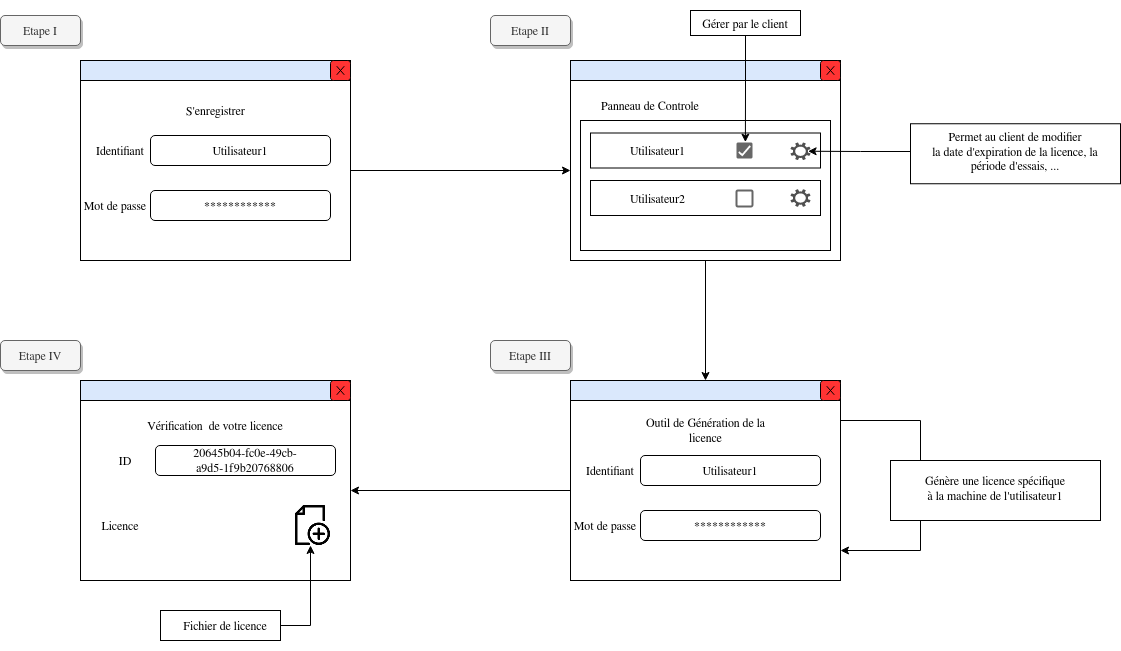
\includegraphics[width=\textwidth]{main/STB.png}
	\caption{Schéma décrivant le fonctionnement général de la solution}
	\label{fig:fig1}
\end{figure}